\documentclass[11pt,a4paper]{article}
\usepackage[a4paper,margin=2.3cm]{geometry}
\usepackage[utf8]{inputenc}
\usepackage[T1]{fontenc}
\IfFileExists{bahasai.ldf}{\usepackage[bahasai]{babel}}{\usepackage[english]{babel}}
\usepackage{booktabs,graphicx,float,amsmath,hyperref,caption,enumitem}
\captionsetup{font=small}
\hypersetup{hidelinks}
\setlist{nosep}
\graphicspath{{figures/}}
\setlength{\parskip}{4pt}\setlength{\parindent}{0pt}\setlength{\emergencystretch}{3em}
% Dibuat otomatis oleh kode/common/make_tables.py — JANGAN diedit manual.

\newcommand{\TduaAdvAUC}{0.873}  % t2_experimen.json
\newcommand{\TduaAdvAUCSebelum}{0.985}  % t2_experimen.json
\newcommand{\TduaBatasLatih}{2025-08-11}  % t2_final.json
\newcommand{\TduaBatasMatang}{2025-08-11}  % t2_audit.json
\newcommand{\TduaBiayaAturan}{69.1}  % t2_experimen.json
\newcommand{\TduaBiayaSemua}{2,567.7}  % t2_experimen.json
\newcommand{\TduaBiayaThr}{81.3}  % t2_experimen.json
\newcommand{\TduaBiayaTidak}{832.5}  % t2_experimen.json
\newcommand{\TduaFinalValBiaya}{67}  % t2_analisis.json
\newcommand{\TduaFinalValPR}{0.774}  % t2_analisis.json
\newcommand{\TduaFraudRate}{0.65}  % t2_audit.json
\newcommand{\TduaImbTerpilih}{tanpa penanganan}  % t2_experimen.json
\newcommand{\TduaKalTerpilih}{sigmoid}  % t2_experimen.json
\newcommand{\TduaKanalBiayaTerbesar}{aplikasi}  % t2_analisis.json
\newcommand{\TduaKanalRecall}{58.1}  % t2_analisis.json
\newcommand{\TduaKonfigAdaptasi}{semua data latih}  % t2_terpilih.json
\newcommand{\TduaKonfigBatas}{2025-08-11}  % t2_terpilih.json
\newcommand{\TduaKonfigImbalance}{tanpa penanganan}  % t2_terpilih.json
\newcommand{\TduaKonfigKalibrasi}{sigmoid}  % t2_terpilih.json
\newcommand{\TduaKonfigLabel}{buang}  % t2_terpilih.json
\newcommand{\TduaNominalFN}{35.5}  % t2_analisis.json
\newcommand{\TduaPRAUCBersih}{0.781}  % t2_audit.json
\newcommand{\TduaPRAUCReview}{0.917}  % t2_audit.json
\newcommand{\TduaPRLogreg}{0.566}  % t2_experimen.json
\newcommand{\TduaPRPerilaku}{0.787}  % t2_experimen.json
\newcommand{\TduaPRTanpaPerilaku}{0.763}  % t2_experimen.json
\newcommand{\TduaRateDasarMingguan}{0.62}  % t2_audit.json
\newcommand{\TduaRateMingguTerakhir}{0.09}  % t2_audit.json
\newcommand{\TduaRecallAturan}{69.8}  % t2_experimen.json
\newcommand{\TduaReviewAUC}{0.894}  % t2_audit.json
\newcommand{\TduaReviewFraudJikaSatu}{30.4}  % t2_audit.json
\newcommand{\TduaReviewPorsiFraud}{79.9}  % t2_audit.json
\newcommand{\TduaReviewRateTest}{1.23}  % t2_audit.json
\newcommand{\TduaReviewRateTrain}{1.71}  % t2_audit.json
\newcommand{\TduaTestDitandai}{1723}  % t2_final.json
\newcommand{\TduaTestPersenDitandai}{1.62}  % t2_final.json
\newcommand{\TduaTestProbRata}{0.745}  % t2_final.json
\newcommand{\TduaValRandomPR}{0.824}  % t2_experimen.json
\newcommand{\TduaValWaktuPR}{0.787}  % t2_experimen.json
\newcommand{\TsatuBasePinbal}{10.21}  % t1_experimen.json
\newcommand{\TsatuBasePinbalNilan}{6.27}  % t1_experimen.json
\newcommand{\TsatuBeratNAPersen}{5.6}  % t1_audit.json
\newcommand{\TsatuCfgTerbaik}{3}  % t1_experimen.json
\newcommand{\TsatuCovGabungan}{0.94}  % t1_experimen.json
\newcommand{\TsatuCovMondrian}{0.94}  % t1_experimen.json
\newcommand{\TsatuCovPilihFdua}{0.919}  % t1_experimen.json
\newcommand{\TsatuCovRawFdua}{0.874}  % t1_experimen.json
\newcommand{\TsatuCovSatuJendela}{0.913}  % t1_experimen.json
\newcommand{\TsatuCovSebelum}{0.891}  % t1_experimen.json
\newcommand{\TsatuDurasiEkstremN}{397}  % t1_audit.json
\newcommand{\TsatuDurasiEkstremPersen}{0.16}  % t1_audit.json
\newcommand{\TsatuDurasiMaks}{25452}  % t1_audit.json
\newcommand{\TsatuFinalValCov}{0.924}  % t1_analisis.json
\newcommand{\TsatuFinalValPinbal}{6.8}  % t1_analisis.json
\newcommand{\TsatuFinalValPinbalNilan}{4.32}  % t1_analisis.json
\newcommand{\TsatuJarakNolPersen}{0.28}  % t1_audit.json
\newcommand{\TsatuJarakSentinelPersen}{0.18}  % t1_audit.json
\newcommand{\TsatuKonfigEncoding}{target encoding out-of-fold}  % t1_terpilih.json
\newcommand{\TsatuKonfigKalibrasi}{CQR gabungan lintas bulan}  % t1_terpilih.json
\newcommand{\TsatuKonfigMitra}{tanpa fitur mitra\_kurir}  % t1_terpilih.json
\newcommand{\TsatuKoreksiCQR}{4.7}  % t1_final.json
\newcommand{\TsatuLayananTerburuk}{hemat}  % t1_analisis.json
\newcommand{\TsatuLayananTerburukPinbal}{8.71}  % t1_analisis.json
\newcommand{\TsatuLgbCov}{0.891}  % t1_experimen.json
\newcommand{\TsatuLgbPinbal}{6.77}  % t1_experimen.json
\newcommand{\TsatuLgbPinbalNilan}{4.29}  % t1_experimen.json
\newcommand{\TsatuLinPinbal}{7.42}  % t1_experimen.json
\newcommand{\TsatuLinPinbalNilan}{4.57}  % t1_experimen.json
\newcommand{\TsatuMedianEkstremBagi}{61.4}  % t1_audit.json
\newcommand{\TsatuMedianNormal}{61.6}  % t1_audit.json
\newcommand{\TsatuMitraSim}{K12}  % t1_experimen.json
\newcommand{\TsatuMitraTerburuk}{K07}  % t1_analisis.json
\newcommand{\TsatuMitraTerburukPinbal}{10.24}  % t1_analisis.json
\newcommand{\TsatuPersenKoreksiMonoton}{0}  % t1_final.json
\newcommand{\TsatuPinbalBersih}{6.85}  % t1_audit.json
\newcommand{\TsatuPinbalScan}{5.4}  % t1_audit.json
\newcommand{\TsatuPinbalScanTest}{10.55}  % t1_audit.json
\newcommand{\TsatuPulauTerburuk}{Papua}  % t1_analisis.json
\newcommand{\TsatuPulauTerburukPinbal}{21.3}  % t1_analisis.json
\newcommand{\TsatuScanKS}{0.92}  % t1_audit.json
\newcommand{\TsatuScanMeanTest}{1.5}  % t1_audit.json
\newcommand{\TsatuScanMeanTrain}{9.7}  % t1_audit.json
\newcommand{\TsatuScanSpearman}{0.77}  % t1_audit.json
\newcommand{\TsatuShapDua}{jarak\_km}  % t1_analisis.json
\newcommand{\TsatuShapSatu}{layanan}  % t1_analisis.json
\newcommand{\TsatuShapTiga}{kota\_tujuan\_te}  % t1_analisis.json
\newcommand{\TsatuTestPlimaMedian}{63.3}  % t1_final.json
\newcommand{\TsatuTestPnilanMedian}{88.1}  % t1_final.json
\newcommand{\TsatuValRandomCov}{0.883}  % t1_experimen.json
\newcommand{\TsatuValRandomPinbal}{6.64}  % t1_experimen.json
\newcommand{\TsatuValWaktuCov}{0.89}  % t1_experimen.json
\newcommand{\TsatuValWaktuPinbal}{6.82}  % t1_experimen.json
\newcommand{\TtigaAnomaliN}{2546}  % t3_final.json
\newcommand{\TtigaAnomaliPersen}{2.12}  % t3_final.json
\newcommand{\TtigaJaccardMin}{0.972}  % t3_stabilitas.json
\newcommand{\TtigaK}{8}  % t3_metode_k.json
\newcommand{\TtigaKelompokTerpenting}{promo \& pembayaran}  % t3_seleksi_fitur.json
\newcommand{\TtigaKonfigK}{8}  % t3_terpilih.json
\newcommand{\TtigaKonfigMetode}{kmeans}  % t3_terpilih.json
\newcommand{\TtigaMetode}{kmeans}  % t3_metode_k.json
\newcommand{\TtigaNARIPerilaku}{-0}  % t3_seleksi_fitur.json
\newcommand{\TtigaNMaxKorelasi}{0.01}  % t3_seleksi_fitur.json
\newcommand{\TtigaNRun}{20}  % t3_stabilitas.json
\newcommand{\TtigaNSegmen}{7}  % t3_final.json
\newcommand{\TtigaNSil}{0.67}  % t3_seleksi_fitur.json
\newcommand{\TtigaSemuaVsN}{0.08}  % t3_seleksi_fitur.json
\newcommand{\TtigaSilK}{0.092}  % t3_metode_k.json
\newcommand{\TtigaStabK}{0.982}  % t3_metode_k.json
\newcommand{\TtigaStabKmin}{0.983}  % t3_metode_k.json
\newcommand{\TtigaStabKplus}{0.869}  % t3_metode_k.json
\newcommand{\TtigaStabMean}{0.985}  % t3_stabilitas.json
\newcommand{\TtigaStabMin}{0.97}  % t3_stabilitas.json
\newcommand{\TtigaStabStd}{0.005}  % t3_stabilitas.json


\title{UTS Machine Learning\\\large Estimasi Waktu Kirim, Deteksi Fraud, dan Segmentasi Pelanggan}
\author{Kelompok 2 \\ Hadi Nugroho (101032330235) \quad Aryo Zaki Abdillah (101032300060)}
\date{November 2026}

\begin{document}
\maketitle

\section{Pendahuluan}
Laporan ini menjawab tiga tugas UTS: (1) regresi waktu kirim paket sebagai median (P50) dan batas atas 90\% (P90),
(2) deteksi fraud transaksi beserta keputusan transaksi mana yang ditinjau, dan (3) segmentasi pelanggan tanpa label.
Tiga prinsip dipegang di seluruh pekerjaan:
\begin{enumerate}
  \item \textbf{Hanya informasi yang tersedia saat prediksi.} Setiap fitur diaudit; fitur yang baru ada setelah kejadian dibuang dengan bukti dan dampak terukur.
  \item \textbf{Validasi meniru pemakaian nyata.} Data uji adalah September--Oktober 2025, sehingga Tugas 1 dan 2 divalidasi dengan skema berbasis waktu (latih di masa lalu, uji 2 bulan berikutnya). Random CV hanya dipakai sebagai pembanding.
  \item \textbf{Reproducibility.} Semua angka di laporan dibaca otomatis dari file hasil di \url{kode/outputs/results/}. Satu perintah menghasilkan ulang seluruh angka, gambar, tabel, dan file prediksi (seed 42):\\ \texttt{python kode/run\_all.py -{}-task all -{}-mode train}
\end{enumerate}
Semua model adalah model klasik (scikit-learn, LightGBM).

\section{Tugas 1 -- Estimasi Waktu Kirim (Regresi P50 dan P90)}
Data latih berisi 250.000 paket yang diambil kurir Januari--Agustus 2025; data uji 60.000 paket September--Oktober 2025.
Target \texttt{durasi\_jam} diprediksi sebagai P50 dan P90 pada saat paket diambil kurir.

\subsection*{(a) Audit data}
\textbf{Kesalahan satuan pada target.} Sebanyak \TsatuDurasiEkstremN{} paket (\TsatuDurasiEkstremPersen\%) memiliki durasi di atas 500 jam
(maksimum \TsatuDurasiMaks{} jam). Jika dibagi 60, median kelompok ini menjadi \TsatuMedianEkstremBagi{} jam, hampir sama dengan median
data normal (\TsatuMedianNormal{} jam) --- bukti kuat bahwa nilai tersebut tercatat dalam menit (Gambar~\ref{fig:t1durasi}).
Tiga perlakuan dibandingkan pada validasi waktu (Tabel~\ref{tab:t1_audit_target}); perlakuan ``dibagi 60'' dipakai.

\textbf{Nilai tidak valid.} \texttt{jarak\_km} bernilai sentinel 9999 (\TsatuJarakSentinelPersen\%) dan 0 (\TsatuJarakNolPersen\%),
juga muncul di data uji, sehingga diubah menjadi \textit{missing} dengan indikator \texttt{jarak\_tidak\_valid}.
\texttt{berat\_kg} kosong pada \TsatuBeratNAPersen\% baris; dibiarkan \textit{missing} (ditangani LightGBM) ditambah indikator.

\textbf{Fitur yang tidak tersedia saat pickup.} Setiap fitur numerik dibandingkan distribusinya antara data latih dan uji (statistik KS)
serta korelasinya dengan target (Tabel~\ref{tab:t1_audit_ks}). \texttt{jumlah\_scan} menonjol: korelasi Spearman dengan durasi
\TsatuScanSpearman{}, tetapi rata-ratanya \TsatuScanMeanTrain{} di data latih dan hanya \TsatuScanMeanTest{} di data uji (KS = \TsatuScanKS).
Scan dicatat \emph{selama} perjalanan; pada saat pickup jumlahnya baru 1--2. \texttt{f30} naik lurus setiap bulan (Gambar~\ref{fig:t1bocor}),
sehingga hanya berfungsi sebagai penanda waktu yang tidak dapat diekstrapolasi ke September--Oktober.

\textbf{Dampak.} Dengan \texttt{jumlah\_scan}, pinball P50 validasi tampak membaik dari \TsatuPinbalBersih{} menjadi \TsatuPinbalScan.
Namun ketika nilai \texttt{jumlah\_scan} diganti dengan distribusi seperti di data uji, pinball P50 memburuk menjadi \TsatuPinbalScanTest{}
dan coverage P90 runtuh (Tabel~\ref{tab:t1_audit_dampak}). Kedua fitur dibuang.

\begin{table}[ht]
\centering\small
\resizebox{\ifdim\width>\linewidth\linewidth\else\width\fi}{!}{%
\begin{tabular}{lrrrr}
\toprule
varian & pinball50 & pinball90 & coverage90 & mae \\
\midrule
tanpa fitur bermasalah (dipakai) & 6.853 & 4.349 & 0.875 & 13.706 \\
+ jumlah\_scan (bocor) & 5.399 & 2.917 & 0.874 & 10.798 \\
+ jumlah\_scan (bocor), nilai seperti di test & 10.545 & 12.338 & 0.441 & 21.090 \\
+ f30 (penanda waktu) & 6.852 & 4.357 & 0.873 & 13.704 \\
\bottomrule
\end{tabular}
}
\caption{Dampak fitur bermasalah pada validasi waktu F2 (latih Jan–Jun, val Jul–Agu).}
\label{tab:t1_audit_dampak}
\end{table}

\begin{figure}[ht]\centering
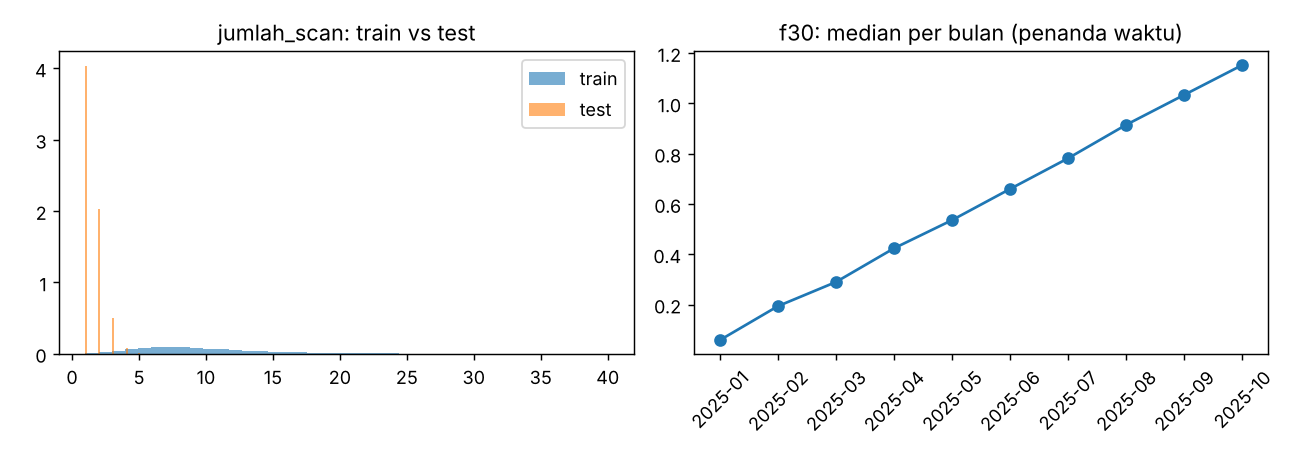
\includegraphics[width=.9\linewidth]{t1_audit_bocor.png}
\caption{Kiri: distribusi \texttt{jumlah\_scan} di data latih vs uji. Kanan: median \texttt{f30} per bulan (penanda waktu).}\label{fig:t1bocor}
\end{figure}

\subsection*{(b) Skema validasi}
Skema utama meniru penggunaan nyata: model dilatih sampai bulan $M$ dan diuji pada dua bulan berikutnya ---
F1 (latih Jan--Apr, uji Mei--Jun) dan F2 (latih Jan--Jun, uji Jul--Agu). Sebagai pembanding, model dan fitur yang sama
dievaluasi dengan random 3-fold CV (Tabel~\ref{tab:t1_validasi}). Random CV memberi pinball P50 rata-rata \TsatuValRandomPinbal{},
lebih optimis dibanding skema waktu (\TsatuValWaktuPinbal), karena model ikut melihat bulan yang sama dengan data uji
(pola musiman dan tren antrean hub). Seluruh tuning dan pemilihan model hanya dilakukan dengan skema waktu.

\begin{table}[ht]
\centering\small
\resizebox{\ifdim\width>\linewidth\linewidth\else\width\fi}{!}{%
\begin{tabular}{llrrrrr}
\toprule
skema & fold & pinball50 & pinball90 & coverage90 & mae & n \\
\midrule
waktu & F1 & 6.795 & 4.216 & 0.906 & 13.590 & 64782 \\
waktu & F2 & 6.853 & 4.349 & 0.875 & 13.706 & 68604 \\
random & R1 & 6.635 & 4.264 & 0.884 & 13.270 & 83334 \\
random & R2 & 6.667 & 4.303 & 0.882 & 13.333 & 83333 \\
random & R3 & 6.631 & 4.242 & 0.882 & 13.263 & 83333 \\
\bottomrule
\end{tabular}
}
\caption{Validasi berbasis waktu vs random 3-fold CV (LightGBM quantile, fitur sama).}
\label{tab:t1_validasi}
\end{table}


\subsection*{(c) Model}
Tiga keluarga model dibandingkan (Tabel~\ref{tab:t1_model}): (i) baseline kuantil empiris per (layanan $\times$ pulau tujuan),
(ii) regresi Ridge dengan target $\log(\text{durasi})$, P90 diperoleh dari kuantil-0,9 residual, dan
(iii) LightGBM dengan \textit{quantile loss} ($\alpha=0{,}5$ dan $\alpha=0{,}9$, dua model terpisah).
Lima konfigurasi LightGBM di-\textit{tune} pada fold waktu (skor = pinball P50 + pinball P90), konfigurasi ke-\TsatuCfgTerbaik{} terbaik.
LightGBM tuned mencapai pinball P50 \TsatuLgbPinbal{} dibanding Ridge \TsatuLinPinbal{} dan baseline \TsatuBasePinbal.

\begin{table}[ht]
\centering\small
\resizebox{\ifdim\width>\linewidth\linewidth\else\width\fi}{!}{%
\begin{tabular}{lrrrr}
\toprule
model & pinball50 & pinball90 & coverage90 & mae \\
\midrule
LightGBM quantile (tuned, cfg 3) & 6.768 & 4.286 & 0.891 & 13.536 \\
LightGBM quantile (default) & 6.824 & 4.282 & 0.890 & 13.648 \\
Linear log-target (Ridge) & 7.417 & 4.571 & 0.913 & 14.834 \\
Baseline kuantil (layanan$\times$pulau) & 10.208 & 6.266 & 0.899 & 20.417 \\
\bottomrule
\end{tabular}
}
\caption{Perbandingan model, rata-rata 2 fold waktu (pinball lebih kecil lebih baik).}
\label{tab:t1_model}
\end{table}


\subsection*{(d) Kategori kardinalitas tinggi dan kategori baru}
\texttt{kota\_tujuan} (405 kategori) dan \texttt{kota\_asal} dibandingkan dengan tiga encoding: target encoding \textit{out-of-fold} dengan smoothing
(dihitung hanya dari data latih fold), frequency encoding, dan kategori native LightGBM (Tabel~\ref{tab:t1_encoding}); terpilih \TsatuKonfigEncoding.
Kategori jarang (< 30 baris) dan kategori yang tidak dikenal dipetakan ke \texttt{\_\_OTHER\_\_}.
Mitra kurir K13 hanya muncul di data uji (±3,9\% baris). Untuk menguji penanganannya, mitra \TsatuMitraSim{} (porsi serupa) dikeluarkan
dari data latih fold F2 lalu diperlakukan sebagai mitra baru (Tabel~\ref{tab:t1_mitra_baru}). Strategi dipilih dengan pinball yang dibobot
porsi mitra baru di data uji; terpilih: \TsatuKonfigMitra.

\begin{table}[ht]
\centering\small
\begin{tabular}{lrrr}
\toprule
encoding kota & pinball50 & pinball90 & coverage90 \\
\midrule
te & 6.832 & 4.356 & 0.874 \\
freq & 6.940 & 4.409 & 0.875 \\
native & 6.845 & 4.385 & 0.873 \\
\bottomrule
\end{tabular}
\caption{Encoding kota\_tujuan/kota\_asal (fold F2).}
\label{tab:t1_encoding}
\end{table}

\begin{table}[ht]
\centering\small
\resizebox{\ifdim\width>\linewidth\linewidth\else\width\fi}{!}{%
\begin{tabular}{lrrrr}
\toprule
strategi & pinball50\_mitra\_baru & coverage90\_mitra\_baru & pinball50\_mitra\_lama & pinball50\_terbobot \\
\midrule
\_\_OTHER\_\_ tanpa dropout & 6.757 & 0.853 & 6.861 & 6.857 \\
\_\_OTHER\_\_ + kategori dropout 5\% & 6.674 & 0.874 & 6.851 & 6.844 \\
tanpa fitur mitra\_kurir & 6.684 & 0.880 & 6.804 & 6.799 \\
\bottomrule
\end{tabular}
}
\caption{Simulasi kategori baru: mitra K12 dikeluarkan dari data latih (fold F2).}
\label{tab:t1_mitra_baru}
\end{table}


\subsection*{(e) Ketidakpastian dan kalibrasi P90}
Model quantile tidak menjamin coverage 90\% bila distribusi bergeser. Kami menerapkan \textit{Conformalized Quantile Regression} (CQR) satu sisi:
skor $s = y - \hat{q}_{0{,}9}$ dihitung pada data \emph{out-of-time}, lalu P90 digeser dengan kuantil-$(1-\alpha)$ skor tersebut.
Kalibrasi dari satu jendela saja ternyata tidak stabil antar fold (Tabel~\ref{tab:t1_kalibrasi}): jendela yang memuat lonjakan Maret membuat koreksi
terlalu besar, sedangkan jendela lain terlalu kecil. Karena itu kami menggabungkan skor dari beberapa jendela bergulir
``latih s.d. bulan $m$, prediksi dua bulan berikutnya'' (horizon yang sama dengan data uji), secara global maupun per layanan (Mondrian).
Pada fold F1 hanya tersedia satu jendela (latih Jan--Feb, kalibrasi Mar--Apr) yang kebetulan memuat lonjakan Maret, sehingga koreksinya
berlebihan --- contoh nyata bahaya kalibrasi dari satu periode. Coverage tanpa kalibrasi juga menurun dari fold ke fold
(Tabel~\ref{tab:t1_kalibrasi}), sehingga risiko \emph{under-coverage} pada September--Oktober nyata.
Aturan pemilihan: dinilai pada fold dengan $\geq 2$ jendela kalibrasi (F2); di antara varian yang pinball P90-nya tidak lebih buruk dari tanpa kalibrasi,
dipilih coverage terdekat 0,90. Pada F2 coverage tanpa kalibrasi \TsatuCovRawFdua{} menjadi \TsatuCovPilihFdua{} dengan varian terpilih
\textbf{\TsatuKonfigKalibrasi}. Gambar~\ref{fig:t1kal} menunjukkan coverage per layanan.

\begin{table}[ht]
\centering\small
\resizebox{\ifdim\width>\linewidth\linewidth\else\width\fi}{!}{%
\begin{tabular}{llrrr}
\toprule
fold & varian & pinball90 & coverage90 & lebar\_median \\
\midrule
F1 & tanpa kalibrasi & 4.216 & 0.907 & 20.941 \\
F1 & CQR jendela terakhir & 4.746 & 0.961 & 34.912 \\
F1 & CQR gabungan lintas bulan & 4.746 & 0.961 & 34.912 \\
F1 & CQR gabungan per layanan & 4.769 & 0.960 & 36.297 \\
F2 & tanpa kalibrasi & 4.356 & 0.874 & 20.017 \\
F2 & CQR jendela terakhir & 4.389 & 0.865 & 18.929 \\
F2 & CQR gabungan lintas bulan & 4.350 & 0.919 & 27.064 \\
F2 & CQR gabungan per layanan & 4.347 & 0.920 & 27.659 \\
\bottomrule
\end{tabular}
}
\caption{Kalibrasi P90 per fold: tanpa kalibrasi, CQR jendela terakhir, CQR gabungan lintas bulan (global / per layanan).}
\label{tab:t1_kalibrasi}
\end{table}

\begin{figure}[ht]\centering
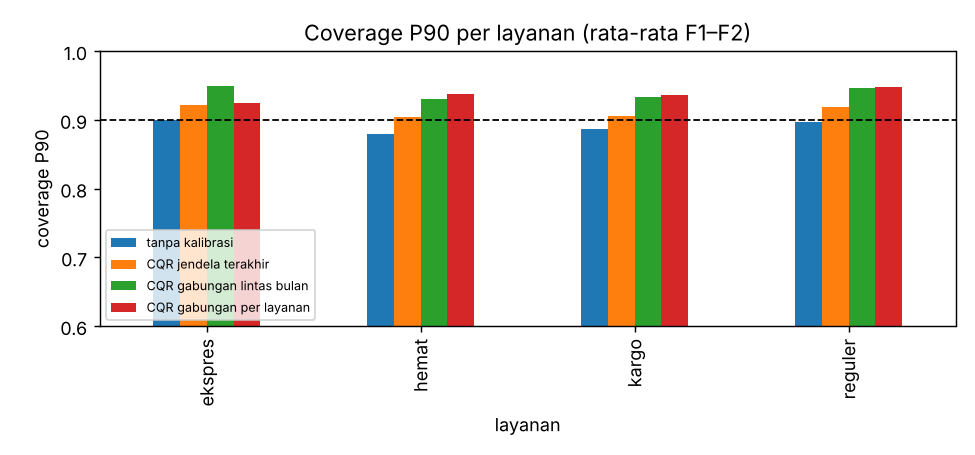
\includegraphics[width=.7\linewidth]{t1_kalibrasi_layanan.png}
\caption{Coverage P90 per layanan untuk tiap varian kalibrasi (rata-rata F1--F2).}\label{fig:t1kal}
\end{figure}

\subsection*{(f) Analisis error dan interpretasi model}
Model final (konfigurasi terpilih + kalibrasi) dievaluasi pada fold F2: pinball P50 \TsatuFinalValPinbal, pinball P90 \TsatuFinalValPinbalNilan,
coverage P90 \TsatuFinalValCov. Error terbesar per layanan terdapat pada \textbf{\TsatuLayananTerburuk} (pinball P50 \TsatuLayananTerburukPinbal),
per pulau tujuan pada \textbf{\TsatuPulauTerburuk} (\TsatuPulauTerburukPinbal), dan per mitra pada \textbf{\TsatuMitraTerburuk} (\TsatuMitraTerburukPinbal)
(Tabel~\ref{tab:t1_breakdown_layanan}--\ref{tab:t1_breakdown_pulau_tujuan}). Error absolut lebih besar pada rute yang durasinya memang panjang;
pola ini konsisten dengan logistik antar-pulau: pengiriman ke Papua (pinball P50 21{,}3 jam) dan Maluku (13{,}8 jam) bergantung pada jadwal kapal atau pesawat yang jarang, sehingga satu jadwal yang terlewat langsung menambah puluhan jam, sedangkan layanan hemat dan kargo lebih sering transit dan menunggu konsolidasi muatan. Mitra K07 perlu perhatian khusus karena coverage P90-nya hanya 0{,}81, jauh di bawah target 0{,}90; artinya model secara sistematis meremehkan durasi mitra ini, sehingga kalibrasi P90 per mitra layak dicoba.
Menurut SHAP (Gambar~\ref{fig:t1shap}), tiga fitur paling berpengaruh pada P50 adalah \texttt{\TsatuShapSatu}, \texttt{\TsatuShapDua}, dan \texttt{\TsatuShapTiga}.
\textit{Partial dependence} (Gambar~\ref{fig:t1pdp}) menunjukkan durasi naik seiring jarak dan antrean hub asal, dengan P90 naik lebih tajam
--- antrean panjang terutama menambah ketidakpastian.

\begin{table}[ht]
\centering\small
\resizebox{\ifdim\width>\linewidth\linewidth\else\width\fi}{!}{%
\begin{tabular}{lrrrrrr}
\toprule
layanan & n & median\_durasi & pinball50 & pinball90 & coverage90 & mae \\
\midrule
hemat & 22760 & 74.500 & 8.706 & 5.065 & 0.915 & 17.412 \\
kargo & 6867 & 79.200 & 7.815 & 4.728 & 0.921 & 15.630 \\
reguler & 28871 & 58.600 & 5.911 & 3.966 & 0.928 & 11.823 \\
ekspres & 10106 & 39.700 & 4.335 & 3.357 & 0.934 & 8.670 \\
\bottomrule
\end{tabular}
}
\caption{Error per layanan (fold F2, model final + kalibrasi).}
\label{tab:t1_breakdown_layanan}
\end{table}

\begin{table}[ht]
\centering\small
\resizebox{\ifdim\width>\linewidth\linewidth\else\width\fi}{!}{%
\begin{tabular}{lrrrrrr}
\toprule
pulau\_tujuan & n & median\_durasi & pinball50 & pinball90 & coverage90 & mae \\
\midrule
Papua & 1226 & 164.050 & 21.304 & 11.220 & 0.888 & 42.608 \\
Maluku & 1341 & 116.500 & 13.759 & 7.037 & 0.915 & 27.518 \\
Kalimantan & 3868 & 92.500 & 11.097 & 6.300 & 0.898 & 22.193 \\
Sulawesi & 4532 & 89.400 & 10.539 & 5.835 & 0.905 & 21.078 \\
Bali-Nusa Tenggara & 2659 & 66.500 & 7.811 & 4.724 & 0.926 & 15.623 \\
Sumatera & 9178 & 64.200 & 7.246 & 4.511 & 0.926 & 14.492 \\
Jawa & 45800 & 56.700 & 5.322 & 3.673 & 0.929 & 10.645 \\
\bottomrule
\end{tabular}
}
\caption{Error per pulau\_tujuan (fold F2, model final + kalibrasi).}
\label{tab:t1_breakdown_pulau_tujuan}
\end{table}

\begin{figure}[ht]\centering
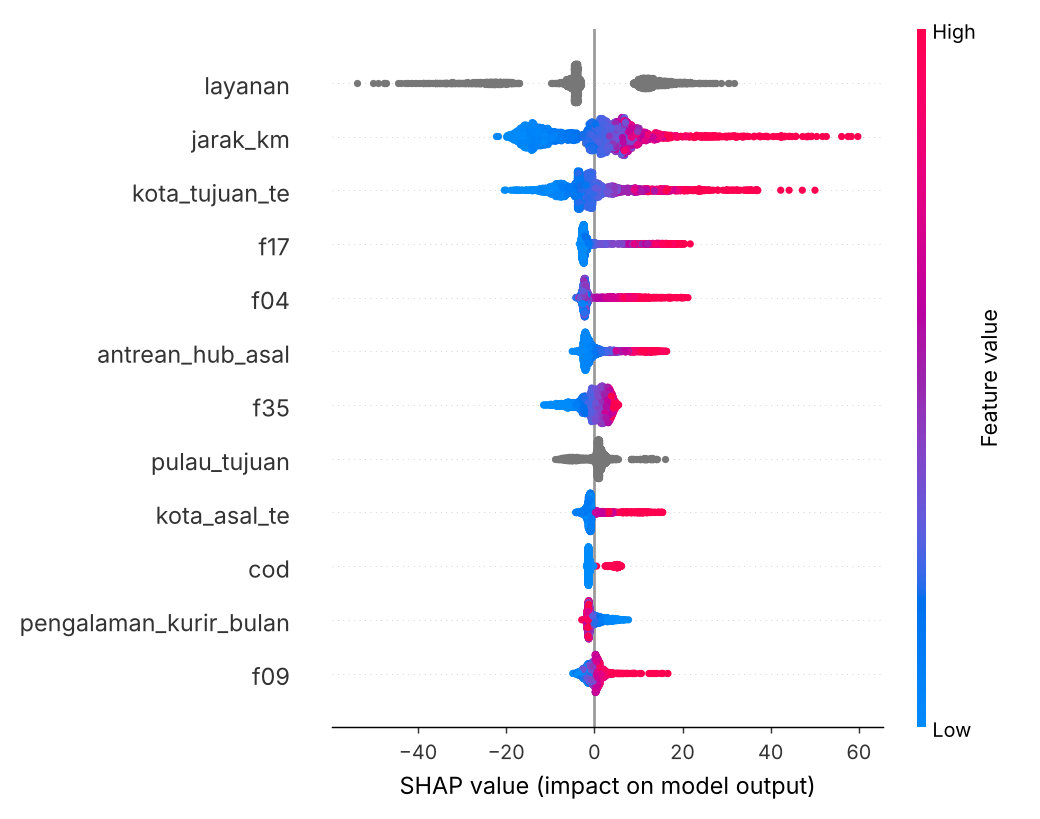
\includegraphics[width=.62\linewidth]{t1_shap_summary.png}
\caption{SHAP summary model P50 (3.000 paket validasi F2).}\label{fig:t1shap}
\end{figure}
\begin{figure}[ht]\centering
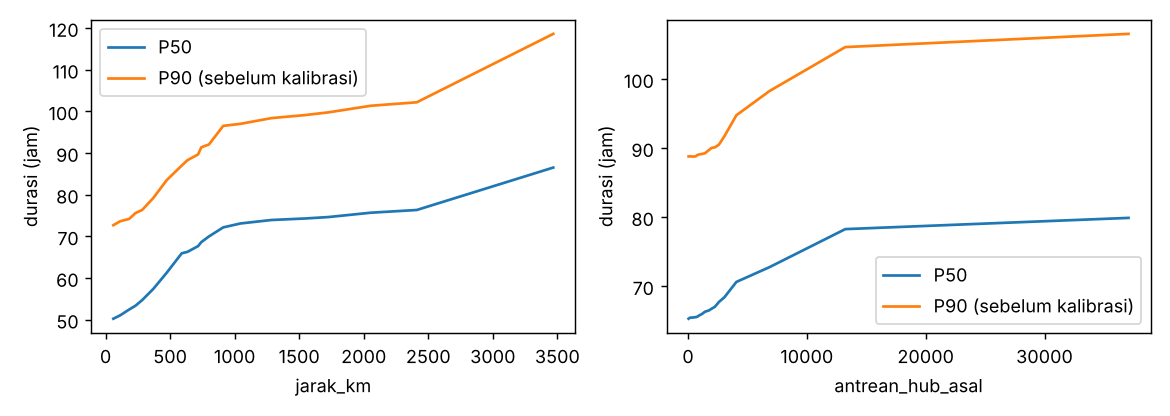
\includegraphics[width=.8\linewidth]{t1_partial_dependence.png}
\caption{Partial dependence P50 dan P90 terhadap jarak dan antrean hub asal.}\label{fig:t1pdp}
\end{figure}

\textbf{Prediksi uji.} Model final dilatih ulang pada Januari--Agustus. Median P50 data uji \TsatuTestPlimaMedian{} jam dan median P90 \TsatuTestPnilanMedian{} jam;
P90 dijamin $\geq$ P50 (koreksi monoton diperlukan pada \TsatuPersenKoreksiMonoton\% paket).

\section{Tugas 2 -- Deteksi Fraud}
Data latih berisi 403.077 transaksi Januari--Agustus 2025 dengan tingkat fraud \TduaFraudRate\%; data uji 106.674 transaksi September--Oktober.
Skor dipakai \emph{sebelum} transaksi diproses, dan setiap transaksi yang ditandai berbiaya Rp~25.000.

\subsection*{(a) Audit label dan fitur}
\textbf{Label belum matang.} Label \texttt{is\_fraud} berarti ``terkonfirmasi fraud saat data ditarik (31 Agustus)''. Tingkat fraud mingguan stabil
di sekitar \TduaRateDasarMingguan\% lalu turun tajam di akhir data hingga \TduaRateMingguTerakhir\% pada minggu terakhir (Gambar~\ref{fig:t2label}):
fraud yang baru terjadi belum sempat dilaporkan sehingga masih berlabel 0. Batas label matang diestimasi otomatis sebagai minggu pertama
yang tingkat fraudnya < 80\% median Januari--Juli: \textbf{\TduaBatasMatang}.

\textbf{Fitur yang tidak tersedia saat transaksi.} \texttt{flag\_review\_manual} memiliki AUC tunggal \TduaReviewAUC: tingkat fraud
\TduaReviewFraudJikaSatu\% pada transaksi yang pernah direview, dan \TduaReviewPorsiFraud\% seluruh fraud pernah direview.
Review dilakukan \emph{setelah} transaksi dicurigai, dan tingkat review di data uji (\TduaReviewRateTest\%) lebih rendah daripada di data latih
(\TduaReviewRateTrain\%) karena sebagian review belum terjadi. Memasukkan fitur ini menaikkan PR-AUC validasi dari \TduaPRAUCBersih{} menjadi
\TduaPRAUCReview{} --- kenaikan semu yang tidak akan terulang di produksi (Tabel~\ref{tab:t2_audit_dampak}). \texttt{v15} naik lurus setiap bulan
(penanda waktu). Keduanya dibuang. Nilai kosong \texttt{menit\_sejak\_trx\_terakhir} dan \texttt{rasio\_nominal\_rata2} (±25\%) terbukti selalu
bersamaan dan menandai transaksi pertama pengguna, sehingga dipertahankan sebagai informasi.

\begin{figure}[ht]\centering
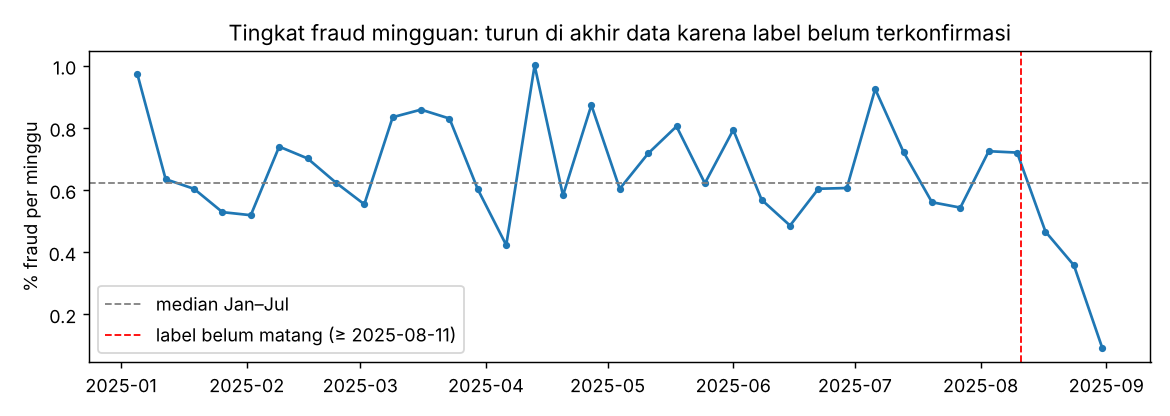
\includegraphics[width=.85\linewidth]{t2_audit_label.png}
\caption{Tingkat fraud mingguan; garis merah = awal periode label belum matang.}\label{fig:t2label}
\end{figure}
\begin{table}[ht]
\centering\small
\begin{tabular}{lrr}
\toprule
varian & pr\_auc & roc\_auc \\
\midrule
tanpa fitur bermasalah (dipakai) & 0.781 & 0.991 \\
+ flag\_review\_manual & 0.917 & 0.997 \\
+ v15 & 0.781 & 0.991 \\
\bottomrule
\end{tabular}
\caption{Dampak fitur bermasalah (fold F2: latih Jan–Mei, val Jun–Jul).}
\label{tab:t2_audit_dampak}
\end{table}


\subsection*{(b) Validasi berbasis waktu dan label yang belum lengkap}
Setiap fold terdiri dari periode latih, satu bulan kalibrasi, dan dua bulan validasi: F1 (latih Jan--Mar, kalibrasi Apr, validasi Mei--Jun) dan
F2 (latih Jan--Apr, kalibrasi Mei, validasi Jun--Jul). Periode validasi sengaja dipilih yang labelnya sudah matang; minggu-minggu akhir Agustus
tidak pernah dipakai sebagai validasi karena fraud-nya belum lengkap dan akan membuat metrik bias.
Random stratified CV memberi PR-AUC \TduaValRandomPR{} dibanding \TduaValWaktuPR{} pada skema waktu (Tabel~\ref{tab:t2_validasi}).

Untuk data latih, kami mensimulasikan kondisi 31 Agustus pada fold F2: fraud di tiga minggu terakhir data latih disembunyikan dengan proporsi
yang sama seperti yang teramati di Agustus, lalu dibandingkan (i) memakai label apa adanya dan (ii) membuang periode belum matang
(Tabel~\ref{tab:t2_label_lag}). Keputusan untuk model final: \textbf{\TduaKonfigLabel} periode belum matang (data latih final sampai \TduaBatasLatih).
Fitur historis berbasis label juga hanya memakai label yang berumur > 30 hari.

\begin{table}[ht]
\centering\small
\resizebox{\ifdim\width>\linewidth\linewidth\else\width\fi}{!}{%
\begin{tabular}{lrrrr}
\toprule
strategi & pr\_auc & roc\_auc & rata2\_prob\_val & fraud\_tersembunyi \\
\midrule
label lengkap (acuan, tidak realistis) & 0.781 & 0.991 & 0.005 & 138 \\
label belum matang dipakai apa adanya & 0.775 & 0.991 & 0.004 & 138 \\
buang periode belum matang (dipakai) & 0.776 & 0.991 & 0.005 & 138 \\
\bottomrule
\end{tabular}
}
\caption{Simulasi label belum matang pada 3 minggu terakhir data latih (fold F2).}
\label{tab:t2_label_lag}
\end{table}


\subsection*{(c) Fitur perilaku tanpa informasi masa depan}
Data latih dan uji digabung lalu diurutkan menurut waktu; setiap fitur hanya memakai transaksi \emph{sebelum} transaksi tersebut.
Fitur pengguna: rata-rata dan z-score log-nominal terhadap riwayatnya, rasio terhadap nominal maksimum sebelumnya, merchant/kategori baru,
jumlah transaksi 1 jam dan 24 jam (hitungan sendiri), jeda sejak transaksi sebelumnya, porsi transaksi malam. Fitur merchant: rasio nominal
terhadap rata-rata merchant, volume 24 jam dan 7 hari, pengguna baru. Tingkat fraud historis merchant dan pengguna dihitung hanya dari label yang
sudah matang (> 30 hari sebelumnya), dengan smoothing. Tiga tes otomatis memastikan tidak ada kebocoran: fitur masa lalu tidak berubah jika data
atau label masa depan diubah, dan hitung ulang manual cocok. Fitur perilaku menaikkan PR-AUC rata-rata dari \TduaPRTanpaPerilaku{} menjadi
\TduaPRPerilaku{} (Tabel~\ref{tab:t2_fitur_perilaku}).

\begin{table}[ht]
\centering\small
\begin{tabular}{lrr}
\toprule
fitur & pr\_auc & roc\_auc \\
\midrule
+ fitur perilaku (dipakai) & 0.787 & 0.990 \\
tanpa fitur perilaku buatan & 0.763 & 0.985 \\
\bottomrule
\end{tabular}
\caption{Dampak fitur perilaku buatan (rata-rata F1–F2).}
\label{tab:t2_fitur_perilaku}
\end{table}


\subsection*{(d) Ketidakseimbangan kelas}
Dibandingkan baseline regresi logistik (PR-AUC \TduaPRLogreg) dan LightGBM dengan empat strategi: tanpa penanganan, \textit{class weight}
(\texttt{scale\_pos\_weight} = $\sqrt{\text{neg}/\text{pos}}$), \textit{undersampling} negatif 1:20, dan SMOTE 1:10 (hanya pada data latih fold).
Karena reweighting dan resampling menggeser probabilitas, setiap varian dikalibrasi isotonic di bulan kalibrasi sebelum aturan biaya diterapkan.
Pendekatan keempat, \textit{threshold tuning}, dibandingkan sebagai kolom ``biaya threshold tunggal'' (Tabel~\ref{tab:t2_imbalance}).
Terpilih: \textbf{\TduaKonfigImbalance} (biaya validasi terendah).

\begin{table}[ht]
\centering\small
\resizebox{\ifdim\width>\linewidth\linewidth\else\width\fi}{!}{%
\begin{tabular}{lrrrrrrr}
\toprule
strategi & pr\_auc & roc\_auc & biaya aturan (juta Rp) & biaya thr tunggal (juta Rp) & recall & presisi & ece\_mentah \\
\midrule
tanpa penanganan & 0.775 & 0.988 & 69.484 & 81.291 & 0.693 & 0.371 & 0.002 \\
undersampling negatif 1:20 & 0.760 & 0.988 & 71.514 & 83.972 & 0.685 & 0.354 & 0.002 \\
class weight (scale\_pos\_weight) & 0.769 & 0.989 & 72.333 & 82.470 & 0.684 & 0.386 & 0.001 \\
SMOTE (rasio 1:10) & 0.769 & 0.986 & 73.953 & 87.238 & 0.685 & 0.363 & 0.001 \\
Logistic regression (baseline) & 0.566 & 0.931 & 128.265 & 157.154 & 0.533 & 0.356 & 0.001 \\
\bottomrule
\end{tabular}
}
\caption{Strategi class imbalance (rata-rata F1–F2). Probabilitas dikalibrasi isotonic di bulan kalibrasi sebelum aturan biaya.}
\label{tab:t2_imbalance}
\end{table}


\subsection*{(e) Pergeseran pola}
Tingkat fraud per kanal berubah dari bulan ke bulan (Gambar~\ref{fig:t2drift}). \textit{Adversarial validation} (Juni--Agustus vs data uji)
menunjukkan model dapat membedakan keduanya dengan AUC \TduaAdvAUCSebelum{}; penyebab utamanya fitur kumulatif sejak Januari (jumlah transaksi,
tingkat fraud kategori kumulatif) yang nilainya naik terus mengikuti waktu. Setelah fitur tersebut dibuang, AUC adversarial turun menjadi
\TduaAdvAUC{} dengan PR-AUC hampir tidak berubah (Tabel~\ref{tab:t2_adversarial}). Adaptasi terhadap pergeseran dibandingkan pada fold F2:
seluruh data, tiga bulan terakhir saja, dan bobot waktu dengan paruh 60 hari (Tabel~\ref{tab:t2_adaptasi}); terpilih \textbf{\TduaKonfigAdaptasi}.

\begin{figure}[ht]\centering
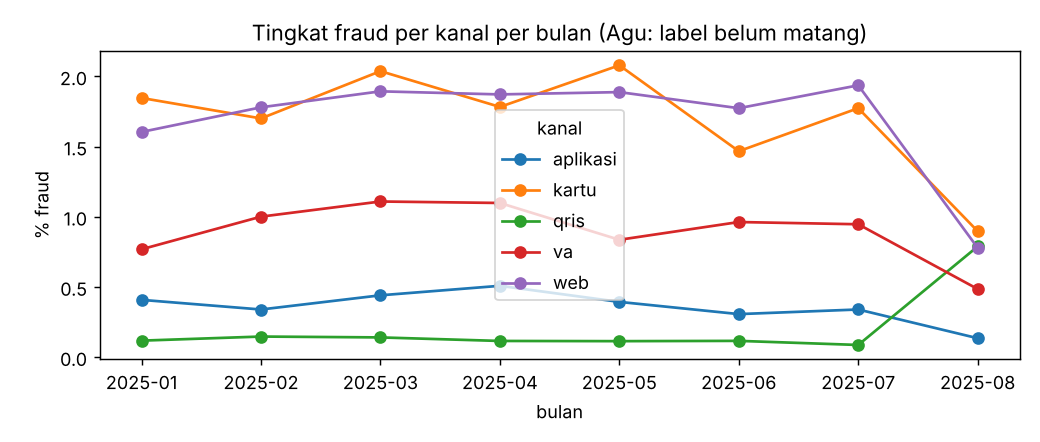
\includegraphics[width=.75\linewidth]{t2_drift_kanal.png}
\caption{Tingkat fraud per kanal per bulan.}\label{fig:t2drift}
\end{figure}
\begin{table}[ht]
\centering\small
\begin{tabular}{lrr}
\toprule
fitur & AUC adversarial (train vs test) & PR-AUC F2 \\
\midrule
dengan fitur kumulatif & 0.985 & 0.784 \\
tanpa fitur kumulatif (dipakai) & 0.873 & 0.781 \\
\bottomrule
\end{tabular}
\caption{Adversarial validation (Jun–Agu vs test Sep–Okt) sebelum/sesudah membuang fitur kumulatif.}
\label{tab:t2_adversarial}
\end{table}

\begin{table}[ht]
\centering\small
\begin{tabular}{lrr}
\toprule
adaptasi & pr\_auc & roc\_auc \\
\midrule
semua data latih & 0.781 & 0.991 \\
3 bulan terakhir saja & 0.769 & 0.990 \\
bobot waktu (paruh 60 hari) & 0.777 & 0.991 \\
\bottomrule
\end{tabular}
\caption{Adaptasi terhadap pergeseran pola (fold F2).}
\label{tab:t2_adaptasi}
\end{table}


\subsection*{(f) Kalibrasi dan aturan keputusan berbasis biaya}
Jika transaksi ditandai, biayanya Rp~25.000 (fraud tertahan tanpa kerugian); jika tidak, ekspektasi kerugiannya $p \times \text{nominal}$.
Maka transaksi ditandai bila $p \times \text{nominal} > 25.000$. Aturan ini hanya benar bila $p$ terkalibrasi, sehingga dibandingkan tanpa kalibrasi,
Platt (sigmoid), dan isotonic pada bulan kalibrasi (Tabel~\ref{tab:t2_kalibrasi_biaya}, Gambar~\ref{fig:t2rel}); terpilih \textbf{\TduaKonfigKalibrasi}.
Rata-rata biaya validasi per dua bulan: aturan kami Rp~\TduaBiayaAturan{} juta (recall \TduaRecallAturan\%), threshold tunggal Rp~\TduaBiayaThr{} juta,
menandai semua Rp~\TduaBiayaSemua{} juta, dan tidak menandai sama sekali Rp~\TduaBiayaTidak{} juta.

\begin{table}[ht]
\centering\small
\resizebox{\ifdim\width>\linewidth\linewidth\else\width\fi}{!}{%
\begin{tabular}{lrrrrrr}
\toprule
kalibrasi & brier & ece & biaya\_aturan\_p\_x\_nominal & biaya\_threshold\_tunggal & biaya\_tandai\_semua & biaya\_tidak\_menandai \\
\midrule
isotonic & 0.0023 & 0.0003 & 69.4844 & 81.2908 & 2567.6875 & 832.4982 \\
none & 0.0024 & 0.0018 & 83.1257 & 81.3297 & 2567.6875 & 832.4982 \\
sigmoid & 0.0022 & 0.0002 & 69.1319 & 81.3297 & 2567.6875 & 832.4982 \\
\bottomrule
\end{tabular}
}
\caption{Kalibrasi (Brier, ECE) dan biaya (juta Rp) di validasi, rata-rata F1–F2.}
\label{tab:t2_kalibrasi_biaya}
\end{table}

\begin{figure}[ht]\centering
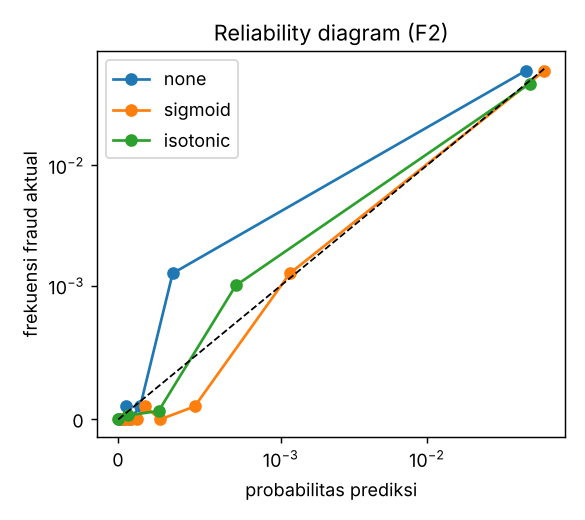
\includegraphics[width=.45\linewidth]{t2_reliability.png}
\caption{Reliability diagram fold F2 (skala log).}\label{fig:t2rel}
\end{figure}

\subsection*{(g) Analisis error}
Pada fold F2 model final mencapai PR-AUC \TduaFinalValPR{} dengan biaya Rp~\TduaFinalValBiaya{} juta, yang sebagian besar berasal dari fraud lolos
senilai Rp~\TduaNominalFN{} juta. Kanal dengan biaya terbesar adalah \textbf{\TduaKanalBiayaTerbesar} (recall \TduaKanalRecall\%)
(Tabel~\ref{tab:t2_breakdown_kanal}). Pola fraud yang ditemukan beserta recall model per pola ada di Tabel~\ref{tab:t2_pola_fraud};
pola dengan porsi terbesar adalah \emph{akun baru ($<$30 hari)}, yaitu 13{,}8\% dari seluruh fraud, tetapi recall model pada pola ini hanya 0{,}48. Dugaan kami, akun baru belum punya riwayat transaksi, sehingga fitur perilaku berbasis riwayat (rata-rata dan frekuensi sebelumnya) belum informatif. Recall terendah ada pada \emph{card testing} (0{,}37): nominalnya kecil ($<$Rp50 ribu), sehingga dengan aturan biaya kerugian per transaksi yang lolos rendah dan banyak yang berada di bawah threshold. Sebaliknya, pola pengambilalihan akun dan kartu tidak hadir jarak jauh tertangkap dengan baik (recall $\geq$0{,}95) karena sinyalnya kuat dan jelas.
\begin{table}[ht]
\centering\small
\resizebox{\ifdim\width>\linewidth\linewidth\else\width\fi}{!}{%
\begin{tabular}{lrrrrrrrrr}
\toprule
kanal & n & n\_fraud & rate\_fraud\_\% & pr\_auc & recall & FN & FP & nominal\_FN\_juta & biaya\_juta \\
\midrule
aplikasi & 45765 & 148 & 0.32 & 0.65 & 0.58 & 62 & 327 & 10.32 & 20.64 \\
kartu & 12676 & 206 & 1.63 & 0.83 & 0.71 & 60 & 154 & 9.08 & 16.58 \\
qris & 22714 & 23 & 0.10 & 0.08 & 0.22 & 18 & 130 & 9.20 & 12.57 \\
va & 15194 & 145 & 0.95 & 0.81 & 0.88 & 18 & 136 & 4.31 & 10.88 \\
web & 6360 & 118 & 1.86 & 0.91 & 0.75 & 30 & 60 & 2.63 & 6.33 \\
\bottomrule
\end{tabular}
}
\caption{Error per kanal (fold F2, aturan biaya).}
\label{tab:t2_breakdown_kanal}
\end{table}

\begin{table}[ht]
\centering\small
\resizebox{\ifdim\width>\linewidth\linewidth\else\width\fi}{!}{%
\begin{tabular}{lrrrr}
\toprule
pola & n\_trx & rate\_fraud\_\% & porsi\_dari\_semua\_fraud\_\% & recall\_model \\
\midrule
akun baru (< 30 hari) & 3551 & 2.48 & 13.75 & 0.48 \\
akses dari IP luar negeri & 861 & 9.06 & 12.19 & 0.68 \\
pengambilalihan akun (ganti password 7h + perangkat baru) & 131 & 51.15 & 10.47 & 0.96 \\
card testing ($\geq$3 trx/1 jam, nominal < 50rb) & 511 & 11.15 & 8.91 & 0.37 \\
kartu tidak hadir + jarak jauh (> 500 km) & 296 & 7.09 & 3.28 & 0.95 \\
merchant refund tinggi (> 10\%) & 31 & 12.90 & 0.62 & 1.00 \\
\bottomrule
\end{tabular}
}
\caption{Pola fraud: tingkat fraud dalam pola, porsi dari seluruh fraud, dan recall model (F2).}
\label{tab:t2_pola_fraud}
\end{table}


\textbf{Prediksi uji.} Model final dilatih sampai \TduaBatasLatih; pada data uji \TduaTestDitandai{} transaksi (\TduaTestPersenDitandai\%) ditandai
untuk direview, dengan rata-rata probabilitas \TduaTestProbRata\%.

\section{Tugas 3 -- Segmentasi Pelanggan}
Data berisi 120.000 pelanggan dengan ringkasan perilaku 90 hari, tanpa label.

\subsection*{(a) Preprocessing}
\begin{itemize}
  \item \textbf{Skala dan skewness.} Variabel uang, hitungan, recency, dan aktivitas sangat menceng ke kanan (mis. \texttt{sesi\_per\_minggu} maks.\ 399,9)
        sehingga ditransformasi $\log(1+x)$, lalu di-\textit{winsorize} pada persentil 0,5--99,5 dan diskalakan dengan \textit{RobustScaler} (rentang persentil 10--90).
  \item \textbf{Data komposisional.} 16 porsi kategori dan 4 porsi waktu belanja masing-masing berjumlah 1; menaikkan satu porsi pasti menurunkan yang lain,
        sehingga jarak Euclidean pada porsi mentah tidak bermakna. Digunakan transformasi \textit{centered log-ratio}:
        $\mathrm{clr}(x)_i = \log(x_i+\varepsilon) - \frac{1}{D}\sum_j \log(x_j+\varepsilon)$, $\varepsilon = 10^{-3}$.
  \item \textbf{Kategorikal.} \texttt{kota\_tier} (ordinal 1--3) dipakai apa adanya; \texttt{perangkat} di-\textit{one-hot}.
  \item \textbf{Missing.} \texttt{rata2\_keranjang} kosong tepat ketika \texttt{frekuensi\_90h} = 0 (missing struktural), sehingga diisi 0 dan ditambah indikator \texttt{tidak\_aktif\_90h}.
  \item \textbf{Outlier dan inkonsistensi.} \texttt{rasio\_konversi} > 1 dan \texttt{belanja\_30h} > \texttt{belanja\_90h} dicatat sebagai inkonsistensi untuk tahap anomali (g).
\end{itemize}

\subsection*{(b) Seleksi dan pembobotan fitur}
\textbf{Kolom n01--n15.} Kamus data hanya menyebut n01--n10, tetapi data berisi 15 kolom. Korelasi Spearman maksimum dengan semua kolom lain hanya \TtigaNMaxKorelasi.
Namun kolom-kolom ini membentuk cluster yang sangat rapi \emph{di antara mereka sendiri} (silhouette \TtigaNSil) yang sama sekali tidak terkait
dengan cluster perilaku (ARI \TtigaNARIPerilaku), perangkat, maupun kota (Tabel~\ref{tab:t3_bukti_n}). Jika ikut dimasukkan, hasil clustering tertarik
ke struktur n (ARI dengan cluster n = \TtigaSemuaVsN; Tabel~\ref{tab:t3_konfigurasi_fitur}). Struktur yang kuat tetapi tidak berhubungan dengan perilaku
belanja tidak dapat ditindaklanjuti oleh tim marketing, sehingga n01--n15 dibuang.

\textbf{Redundansi dan bobot.} \texttt{belanja\_30h}/\texttt{frekuensi\_30h} berkorelasi tinggi dengan versi 90 harinya tetapi tetap dipakai sebagai sinyal tren terbaru.
Fitur dikelompokkan (RFM, kategori, waktu belanja, promo \& pembayaran, perilaku pasca-beli, aktivitas aplikasi, profil), dan setiap kolom diberi bobot
$1/\sqrt{n_{\text{kelompok}}}$ agar kelompok dengan banyak kolom (16 porsi kategori) tidak mendominasi jarak. Kepentingan tiap kelompok diukur dengan permutasi:
seberapa banyak label berubah jika kelompok diacak (Tabel~\ref{tab:t3_kepentingan_kelompok}); kelompok terpenting: \TtigaKelompokTerpenting.

\begin{table}[ht]
\centering\small
\begin{tabular}{p{0.75\linewidth}r}
\toprule
bukti & nilai \\
\midrule
max\_abs\_spearman\_n\_vs\_perilaku & 0.010 \\
max\_MI\_berlebih\_vs\_acuan\_acak & 0.025 \\
silhouette\_cluster\_n\_saja & 0.670 \\
ARI(cluster\_n, cluster\_perilaku) & -0.000 \\
ARI(cluster\_semua\_kolom, cluster\_n) & 0.083 \\
ARI(cluster\_semua\_kolom, cluster\_perilaku) & 0.398 \\
jumlah\_kolom\_n & 15.000 \\
ARI(cluster\_n, kota\_tier) & -0.000 \\
ARI(cluster\_n, perangkat) & -0.000 \\
\bottomrule
\end{tabular}
\caption{Bukti bahwa n01–n15 membentuk struktur sendiri yang tidak terkait perilaku/profil pelanggan.}
\label{tab:t3_bukti_n}
\end{table}

\begin{table}[ht]
\centering\small
\resizebox{\ifdim\width>\linewidth\linewidth\else\width\fi}{!}{%
\begin{tabular}{lrrrr}
\toprule
konfigurasi & n\_fitur & silhouette & stabilitas\_ARI & ARI\_dengan\_cluster\_n \\
\midrule
semua kolom termasuk n01–n15 & 62 & 0.079 & 0.706 & 0.083 \\
tanpa n, tanpa bobot & 47 & 0.085 & 0.746 & -0.000 \\
tanpa n, bobot per kelompok (dipakai) & 47 & 0.092 & 0.984 & -0.000 \\
\bottomrule
\end{tabular}
}
\caption{Konfigurasi fitur pada k=8: silhouette, stabilitas, dan seberapa jauh cluster ditarik oleh n01–n15.}
\label{tab:t3_konfigurasi_fitur}
\end{table}


\subsection*{(c)--(d) Metode dan jumlah cluster}
Kriteria untuk $k = 2,\dots,12$ (K-Means) ditunjukkan pada Gambar~\ref{fig:t3k} dan Tabel~\ref{tab:t3_kriteria_k}. Silhouette hampir datar (±0,09) dan BIC
terus turun, sehingga keduanya tidak dapat memilih $k$. Stabilitas (rata-rata ARI antar run subsampling 80\%) justru sangat informatif: hanya beberapa $k$
yang menghasilkan partisi konsisten. Aturan yang ditetapkan: \emph{$k$ terbesar dengan stabilitas $\geq 0{,}95$}. Terpilih $k = \TtigaK$
(stabilitas \TtigaStabK, sedangkan $k-1$: \TtigaStabKmin{} dan $k+1$: \TtigaStabKplus). Aturan ``terbesar'' dipilih karena
partisi stabil yang lebih rinci memisahkan kelompok yang benar-benar berbeda; salah satu cluster tambahan pada $k=\TtigaK$
ternyata kelompok berprofil bot yang kemudian diberi label $-1$ (butir g). Stabilitas memakai \texttt{n\_init} = 5 yang sama dengan model final.

Empat metode dibandingkan pada $k$ tersebut (Tabel~\ref{tab:t3_metode}): K-Means, Gaussian Mixture (kovarians diagonal), Agglomerative Ward
(sampel 15.000, sisanya di-assign ke centroid terdekat), dan HDBSCAN (menentukan jumlah cluster sendiri). Terpilih \textbf{\TtigaKonfigMetode}, metode
paling stabil antar seed. HDBSCAN hanya menemukan kelompok berkepadatan berbeda (pelanggan aktif vs tidak aktif) karena segmen lain tidak dipisahkan oleh celah kepadatan.

\begin{figure}[ht]\centering
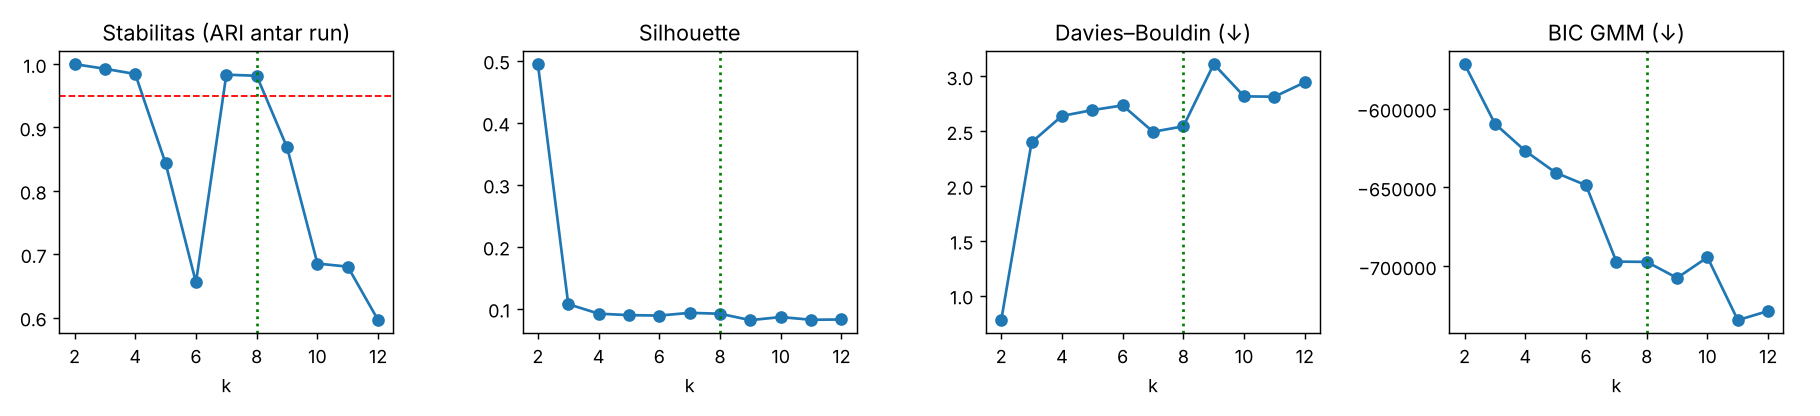
\includegraphics[width=\linewidth]{t3_kriteria_k.png}
\caption{Kriteria jumlah cluster; garis hijau = $k$ terpilih.}\label{fig:t3k}
\end{figure}
\begin{table}[ht]
\centering\small
\resizebox{\ifdim\width>\linewidth\linewidth\else\width\fi}{!}{%
\begin{tabular}{lrrrrrr}
\toprule
metode & n\_cluster & persen\_noise & silhouette & davies\_bouldin & ARI\_antar\_seed & ARI\_vs\_kmeans \\
\midrule
kmeans & 8 & 0.000 & 0.092 & 2.545 & 0.989 & 1.000 \\
gmm & 8 & 0.000 & 0.073 & 3.063 & 0.534 & 0.289 \\
agglomerative & 8 & 0.000 & 0.086 & 2.605 & 0.482 & 0.511 \\
hdbscan & 2 & 0.783 & 0.494 & 0.775 & 0.931 & 0.045 \\
\bottomrule
\end{tabular}
}
\caption{Perbandingan metode pada k=8 (HDBSCAN menentukan jumlah cluster sendiri).}
\label{tab:t3_metode}
\end{table}


\subsection*{(e) Stabilitas}
Clustering akhir diulang \TtigaNRun{} kali pada subsampel 80\% yang berbeda, lalu setiap hasil di-\textit{predict} ke seluruh data.
ARI antar run: rata-rata \TtigaStabMean{} (simpangan baku \TtigaStabStd, minimum \TtigaStabMin). Jaccard terendah per cluster \TtigaJaccardMin{}
(Tabel~\ref{tab:t3_stabilitas}, Gambar~\ref{fig:t3stab}), sehingga semua segmen muncul konsisten.

\begin{table}[ht]
\centering\small
\resizebox{\ifdim\width>\linewidth\linewidth\else\width\fi}{!}{%
\begin{tabular}{rlrrrr}
\toprule
k & metode & n\_run & ARI\_mean & ARI\_std & ARI\_min \\
\midrule
7 & kmeans & 6 & 0.984 & 0.004 & 0.973 \\
8 & kmeans & 20 & 0.985 & 0.005 & 0.970 \\
9 & kmeans & 6 & 0.888 & 0.136 & 0.690 \\
\bottomrule
\end{tabular}
}
\caption{Stabilitas: ARI antar run subsampling 80\% (20 run untuk k=8).}
\label{tab:t3_stabilitas}
\end{table}

\begin{figure}[ht]\centering
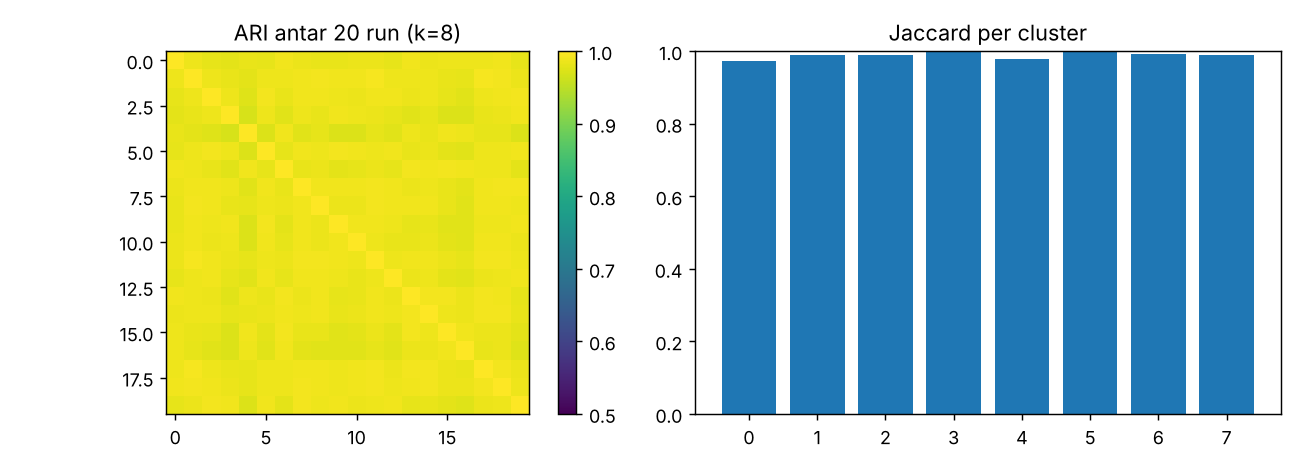
\includegraphics[width=.8\linewidth]{t3_stabilitas.png}
\caption{Kiri: ARI antar run. Kanan: Jaccard tiap cluster terhadap pasangan terdekat di run lain.}\label{fig:t3stab}
\end{figure}

\subsection*{(f) Profil segmen dan aksi marketing}
Terdapat \TtigaNSegmen{} segmen (di luar anomali). Profil median pada fitur asli ada di Tabel~\ref{tab:t3_profil} dan pola pembedanya di Gambar~\ref{fig:t3heat}.
Nama dan aksi per segmen (Tabel~\ref{tab:t3_aksi}) diturunkan dari fitur yang paling membedakan segmen tersebut dari populasi.
Nama segmen hasil otomatis kami cocokkan dengan Tabel~\ref{tab:t3_profil}; dua nama kami ubah agar sesuai profil (segmen~5 menjadi \emph{Pelanggan Loyal Bernilai Tinggi} karena frekuensi dan nilai belanjanya tertinggi, segmen~2 menjadi \emph{Mulai Pasif}). Alasan aksi per segmen: segmen~0 paling sering membeli saat flash sale (69\%), sehingga voucher dengan minimum belanja sedikit di atas keranjangnya dapat menaikkan nilai transaksi; segmen~1 dominan berbelanja pagi hari, sehingga promo dan pengingat dikirim sebelum jam kerja; segmen~2 baru terakhir belanja rata-rata 44 hari lalu, sehingga perlu win-back sebelum benar-benar berhenti; segmen~3 memakai paylater paling tinggi (62\%) di kategori fashion yang rawan retur, sehingga panduan ukuran dan ulasan dapat menekan retur; segmen~4 hampir seluruhnya pengguna iOS dengan belanja besar (Rp3{,}4 juta), cocok untuk produk premium; segmen~5 sudah loyal, sehingga fokusnya menambah nilai lewat cross-sell, bukan diskon; segmen~6 tidak bertransaksi dalam 90 hari, sehingga perlu reaktivasi dengan voucher comeback.
\begin{table}[ht]
\centering\small
\resizebox{\ifdim\width>\linewidth\linewidth\else\width\fi}{!}{%
\begin{tabular}{rrrrrrrlll}
\toprule
segmen & ukuran\_\% & frekuensi\_90h & belanja\_90h (ribu Rp) & recency\_hari & persen\_paylater & persen\_flash\_sale & kategori\_dominan & jam\_dominan & perangkat\_dominan \\
\midrule
0 & 22.70 & 7.00 & 706.60 & 9.20 & 0.17 & 0.69 & fashion & malam & android (74\%) \\
1 & 17.16 & 11.00 & 2690.90 & 6.50 & 0.11 & 0.21 & makanan\_minuman & pagi & android (91\%) \\
2 & 16.63 & 2.00 & 350.55 & 44.20 & 0.17 & 0.30 & makanan\_minuman & sore & android (70\%) \\
3 & 15.52 & 7.00 & 1005.70 & 9.30 & 0.62 & 0.58 & fashion & malam & android (74\%) \\
4 & 14.48 & 8.00 & 3421.80 & 7.50 & 0.10 & 0.17 & makanan\_minuman & siang & ios (96\%) \\
5 & 7.84 & 27.00 & 6741.35 & 6.60 & 0.12 & 0.25 & makanan\_minuman & pagi & android (66\%) \\
6 & 5.67 & 0.00 & 0.00 & 38.50 & 0.17 & 0.33 & makanan\_minuman & malam & android (68\%) \\
\bottomrule
\end{tabular}
}
\caption{Profil segmen (median fitur asli).}
\label{tab:t3_profil}
\end{table}

\begin{table}[ht]
\centering\small
\begin{tabular}{rp{0.23\linewidth}p{0.52\linewidth}}
\toprule
segmen & nama & aksi marketing \\
\midrule
0 & Pemburu Voucher \& Pemburu Flash Sale & voucher bertarget dengan minimum belanja sedikit di atas rata-rata keranjangnya \\
1 & Belanja Pagi \& Pengguna Android & promo pagi hari dan pengingat keranjang sebelum jam kerja \\
2 & Mulai Pasif \& Setia COD & kampanye win-back dengan voucher terbatas waktu \\
3 & Sering Retur \& Pengguna Paylater & panduan ukuran/ulasan produk dan rekomendasi yang lebih akurat \\
4 & Pengguna iOS \& Usia Matang & kampanye produk premium di aplikasi iOS \\
5 & Cepat Membeli \& Rajin Mengulas & rekomendasi produk pelengkap (cross-sell) \\
6 & Pelanggan Tidur & kampanye reaktivasi: voucher comeback + pengingat kategori favorit \\
\bottomrule
\end{tabular}
\caption{Nama segmen dan usulan aksi marketing.}
\label{tab:t3_aksi}
\end{table}

\begin{figure}[ht]\centering
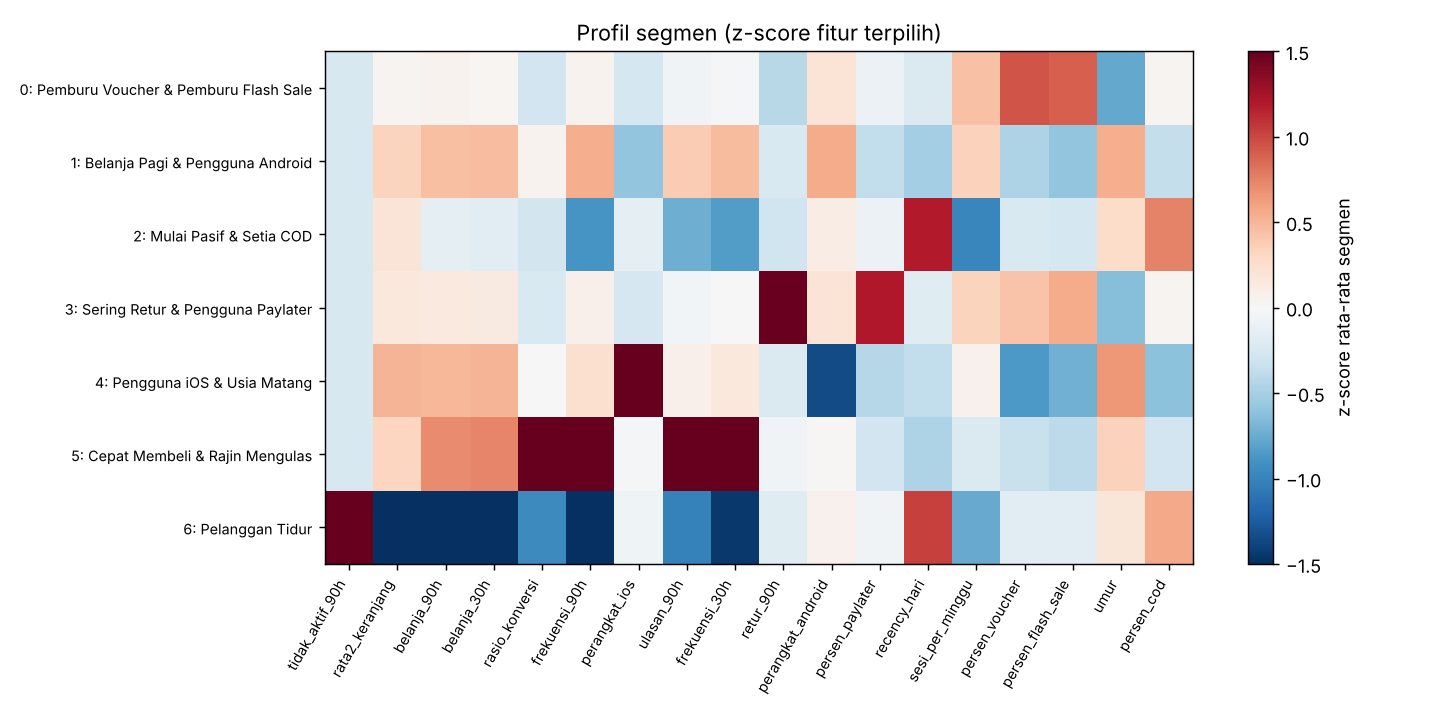
\includegraphics[width=.9\linewidth]{t3_profil_heatmap.png}
\caption{Z-score rata-rata fitur pembeda per segmen.}\label{fig:t3heat}
\end{figure}

\subsection*{(g) Anomali}
Pelanggan diberi label $-1$ bila perilakunya tidak mungkin atau tidak wajar untuk manusia --- lebih dari 100 sesi per minggu (±14 sesi per hari),
rasio konversi > 1, atau belanja 30 hari melebihi belanja 90 hari --- atau bila termasuk cluster yang mayoritas anggotanya melanggar aturan tersebut
(cluster berprofil bot: ratusan sesi per minggu dengan konversi hampir nol). Total \TtigaAnomaliN{} pelanggan (\TtigaAnomaliPersen\%).
Isolation Forest, likelihood GMM, dan jarak ke centroid dibandingkan sebagai alternatif (Tabel~\ref{tab:t3_anomali}); irisannya dengan aturan domain kecil,
artinya detektor statistik umum lebih banyak menandai pelanggan yang sekadar ekstrem namun wajar. Karena pelanggan normal yang diberi $-1$
menurunkan ARI, kami memilih definisi yang konservatif dan dapat dijelaskan.

\begin{table}[ht]
\centering\small
\begin{tabular}{lrrr}
\toprule
metode & jumlah & persen & irisan\_dgn\_aturan\_domain\_\% \\
\midrule
aturan domain & 2426 & 2.022 & 100.000 \\
cluster berprofil bot & 1711 & 1.426 & 92.987 \\
Isolation Forest (top 2\%) & 2400 & 2.000 & 7.750 \\
log-likelihood GMM terendah 2\% & 2400 & 2.000 & 13.875 \\
jarak ke centroid tertinggi 2\% & 2400 & 2.000 & 13.667 \\
\bottomrule
\end{tabular}
\caption{Perbandingan detektor anomali. Label -1 = aturan domain $\cup$ cluster berprofil bot.}
\label{tab:t3_anomali}
\end{table}



\section{Kesimpulan dan Keterbatasan}
\begin{itemize}
  \item \textbf{Tugas 1.} Audit menemukan kebocoran yang paling menentukan (\texttt{jumlah\_scan}) dan kesalahan satuan pada target. Validasi waktu lebih pesimis
        (dan lebih jujur) daripada random CV. LightGBM quantile dengan kalibrasi CQR memberi P50 dan P90 terbaik.
        \textit{Keterbatasan:} distribusi durasi bergeser antar bulan (musim, antrean hub), sehingga coverage P90 pada September--Oktober tetap bergantung pada
        seberapa mirip bulan tersebut dengan jendela kalibrasi.
  \item \textbf{Tugas 2.} Dua hal paling penting adalah menangani label yang belum matang dan membuang fitur yang baru ada setelah transaksi (\texttt{flag\_review\_manual}).
        Keputusan berbasis biaya dengan probabilitas terkalibrasi jauh lebih murah daripada menandai semua atau tidak menandai.
        \textit{Keterbatasan:} pola fraud dan prevalensinya bisa berubah di September--Oktober; kalibrasi perlu diperbarui secara berkala.
  \item \textbf{Tugas 3.} Kolom anonim n01--n15 membentuk struktur kuat yang tidak berkaitan dengan perilaku, sehingga dibuang. Jumlah segmen dipilih dengan stabilitas,
        karena silhouette dan BIC tidak informatif pada data ini. \textit{Keterbatasan:} segmen berbeda secara gradual (silhouette rendah), sehingga pelanggan di
        perbatasan segmen dapat berpindah bila fitur atau bobot diubah.
\end{itemize}


\appendix
\section{Lampiran}
\subsection*{A. Reproduksi}
\begin{verbatim}
pip install -r kode/requirements.txt
python -m pytest -q kode/tests
python kode/run_all.py --task all --mode train
python kode/run_all.py --task t1 --mode reproduce
\end{verbatim}
Perintah ketiga menghasilkan semua angka, gambar, tabel, dan tiga file prediksi; perintah keempat mereproduksi
angka kunci dari model tersimpan dalam kurang dari satu menit. Seed 42. Versi library tercatat di setiap \url{kode/outputs/results/*.json}. Seluruh angka laporan berasal dari
\url{kode/outputs/tables/angka.tex} yang dibuat otomatis dari file hasil.

\subsection*{B. Penggunaan AI}
Kode disusun dengan bantuan Claude (Anthropic). Kelompok memverifikasi hasilnya dengan tes otomatis (metrik dan anti-kebocoran fitur),
membandingkan skema validasi, menjalankan ulang \texttt{-{}-mode reproduce}, dan memeriksa setiap tabel serta gambar. Rincian per anggota ada di \texttt{kontribusi.md}.

\subsection*{C. Tabel dan gambar tambahan}
\begin{figure}[H]\centering
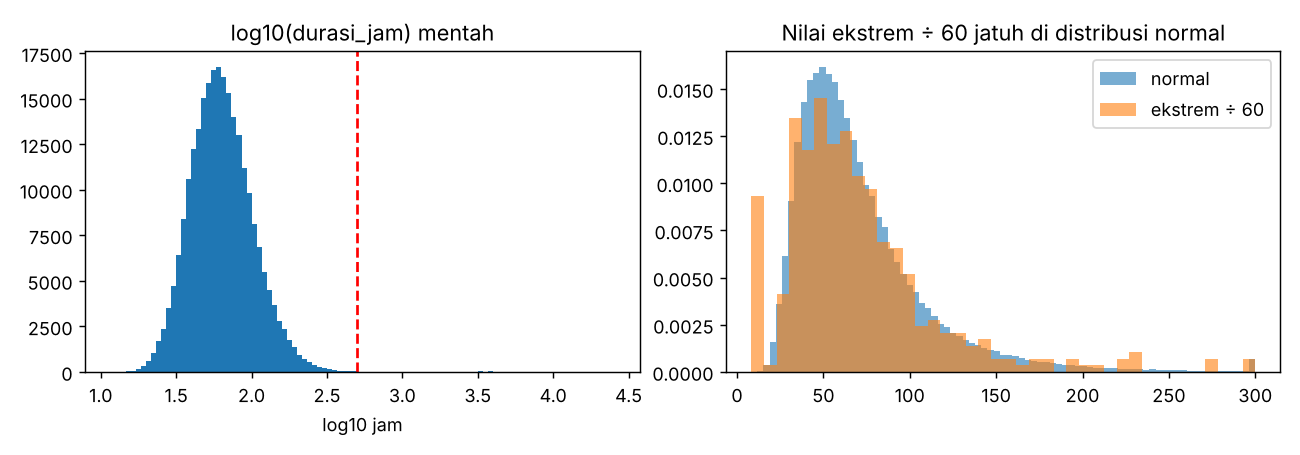
\includegraphics[width=.85\linewidth]{t1_audit_durasi.png}
\caption{Tugas 1: durasi ekstrem (> 500 jam) setelah dibagi 60 jatuh di distribusi normal.}\label{fig:t1durasi}
\end{figure}
\begin{table}[ht]
\centering\small
\resizebox{\ifdim\width>\linewidth\linewidth\else\width\fi}{!}{%
\begin{tabular}{lrrrr}
\toprule
fitur & KS & Spearman & mean\_train & mean\_test \\
\midrule
jumlah\_scan & 0.915 & 0.771 & 9.651 & 1.502 \\
antrean\_hub\_asal & 0.263 & 0.177 & 3328.677 & 4618.876 \\
f30 & 0.232 & -0.004 & 0.497 & 1.092 \\
f17 & 0.108 & 0.215 & 0.264 & 0.346 \\
f35 & 0.092 & 0.106 & 1.006 & 1.029 \\
hujan\_tujuan\_mm & 0.036 & 0.031 & 7.998 & 7.307 \\
hujan\_asal\_mm & 0.033 & 0.019 & 7.925 & 7.289 \\
f24 & 0.010 & 0.001 & 0.004 & -0.008 \\
\bottomrule
\end{tabular}
}
\caption{Fitur dengan beda distribusi train–test terbesar (KS) dan korelasi Spearman dengan durasi.}
\label{tab:t1_audit_ks}
\end{table}

\begin{table}[ht]
\centering\small
\begin{tabular}{lrrr}
\toprule
perlakuan & pinball50 & pinball90 & coverage90 \\
\midrule
bagi60 & 6.853 & 4.349 & 0.875 \\
buang & 6.851 & 4.354 & 0.873 \\
biarkan & 6.924 & 4.376 & 0.877 \\
\bottomrule
\end{tabular}
\caption{Perlakuan durasi ekstrem (> 500 jam), dievaluasi pada label yang sudah dikoreksi.}
\label{tab:t1_audit_target}
\end{table}

\begin{table}[ht]
\centering\small
\resizebox{\ifdim\width>\linewidth\linewidth\else\width\fi}{!}{%
\begin{tabular}{rrrrr}
\toprule
cfg & pinball50 & pinball90 & coverage90 & skor \\
\midrule
0 & 6.824 & 4.282 & 0.890 & 11.106 \\
1 & 6.832 & 4.271 & 0.895 & 11.103 \\
2 & 6.808 & 4.335 & 0.885 & 11.143 \\
3 & 6.768 & 4.286 & 0.891 & 11.054 \\
4 & 6.757 & 4.326 & 0.882 & 11.084 \\
\bottomrule
\end{tabular}
}
\caption{Tuning LightGBM pada fold waktu (skor = pinball50 + pinball90).}
\label{tab:t1_tuning}
\end{table}

\begin{table}[ht]
\centering\small
\resizebox{\ifdim\width>\linewidth\linewidth\else\width\fi}{!}{%
\begin{tabular}{lrrrrrr}
\toprule
mitra\_kurir & n & median\_durasi & pinball50 & pinball90 & coverage90 & mae \\
\midrule
K07 & 5448 & 77.800 & 10.236 & 5.327 & 0.806 & 20.473 \\
K02 & 8309 & 66.200 & 6.901 & 4.328 & 0.921 & 13.802 \\
K03 & 7621 & 64.800 & 6.837 & 4.372 & 0.921 & 13.674 \\
K10 & 4179 & 63.000 & 6.779 & 4.399 & 0.928 & 13.558 \\
K12 & 2808 & 62.500 & 6.692 & 4.232 & 0.927 & 13.384 \\
K06 & 5403 & 62.800 & 6.638 & 4.420 & 0.934 & 13.277 \\
K05 & 6197 & 62.900 & 6.516 & 4.115 & 0.931 & 13.032 \\
K04 & 6777 & 59.700 & 6.344 & 4.215 & 0.941 & 12.688 \\
K11 & 3392 & 60.800 & 6.308 & 4.114 & 0.938 & 12.615 \\
K09 & 4072 & 58.500 & 6.273 & 4.298 & 0.938 & 12.546 \\
K01 & 9621 & 57.700 & 6.211 & 4.086 & 0.943 & 12.423 \\
K08 & 4777 & 52.300 & 5.866 & 3.955 & 0.957 & 11.732 \\
\bottomrule
\end{tabular}
}
\caption{Error per mitra\_kurir (fold F2, model final + kalibrasi).}
\label{tab:t1_breakdown_mitra_kurir}
\end{table}

\begin{table}[ht]
\centering\small
\begin{tabular}{lr}
\toprule
fitur & mean |SHAP| \\
\midrule
layanan & 11.504 \\
jarak\_km & 8.954 \\
kota\_tujuan\_te & 5.972 \\
f17 & 3.789 \\
f04 & 3.449 \\
antrean\_hub\_asal & 2.671 \\
f35 & 2.450 \\
pulau\_tujuan & 2.060 \\
kota\_asal\_te & 2.017 \\
cod & 2.004 \\
\bottomrule
\end{tabular}
\caption{Rata-rata |SHAP| model P50 (3.000 sampel validasi).}
\label{tab:t1_shap}
\end{table}

\begin{table}[ht]
\centering\small
\resizebox{\ifdim\width>\linewidth\linewidth\else\width\fi}{!}{%
\begin{tabular}{llrrr}
\toprule
skema & fold & pr\_auc & roc\_auc & n\_fraud \\
\midrule
waktu & F1 & 0.792 & 0.988 & 666 \\
waktu & F2 & 0.781 & 0.991 & 640 \\
random & R1 & 0.827 & 0.989 & 793 \\
random & R2 & 0.816 & 0.988 & 792 \\
random & R3 & 0.829 & 0.994 & 792 \\
\bottomrule
\end{tabular}
}
\caption{Validasi berbasis waktu (label matang) vs random stratified 3-fold.}
\label{tab:t2_validasi}
\end{table}

\begin{table}[ht]
\centering\small
\begin{tabular}{lr}
\toprule
fitur & porsi gain \\
\midrule
perangkat\_baru & 0.097 \\
menit\_sejak\_trx\_terakhir & 0.076 \\
m\_trx\_7h & 0.075 \\
nominal & 0.067 \\
kategori\_merchant & 0.057 \\
trx\_1j & 0.057 \\
refund\_merchant\_30h & 0.050 \\
persen\_saldo & 0.046 \\
umur\_akun\_hari & 0.037 \\
gagal\_login\_24j & 0.034 \\
\bottomrule
\end{tabular}
\caption{10 fitur terpenting (gain) model F2.}
\label{tab:t2_importance}
\end{table}

\begin{table}[ht]
\centering\small
\resizebox{\ifdim\width>\linewidth\linewidth\else\width\fi}{!}{%
\begin{tabular}{lrrrrrrrrr}
\toprule
kategori\_merchant & n & n\_fraud & rate\_fraud\_\% & pr\_auc & recall & FN & FP & nominal\_FN\_juta & biaya\_juta \\
\midrule
elektronik & 11007 & 93 & 0.84 & 0.78 & 0.83 & 16 & 263 & 11.21 & 19.71 \\
fashion & 6992 & 50 & 0.72 & 0.29 & 0.36 & 32 & 90 & 9.21 & 11.91 \\
gadget & 4262 & 78 & 1.83 & 0.82 & 0.92 & 6 & 155 & 3.24 & 8.91 \\
kecantikan & 4439 & 29 & 0.65 & 0.20 & 0.17 & 24 & 56 & 4.96 & 6.49 \\
voucher\_game & 4830 & 106 & 2.19 & 0.91 & 0.79 & 22 & 19 & 1.19 & 3.77 \\
emas & 1611 & 39 & 2.42 & 0.85 & 0.97 & 1 & 91 & 0.12 & 3.35 \\
toko\_online & 8267 & 64 & 0.77 & 0.83 & 0.47 & 34 & 30 & 1.67 & 3.17 \\
top\_up\_ewallet & 5325 & 59 & 1.11 & 0.94 & 0.92 & 5 & 30 & 0.96 & 3.06 \\
pulsa\_data & 9648 & 73 & 0.76 & 0.87 & 0.48 & 38 & 7 & 0.66 & 1.71 \\
rumah\_tangga & 3959 & 5 & 0.13 & 0.56 & 0.60 & 2 & 2 & 0.93 & 1.05 \\
hotel & 3695 & 6 & 0.16 & 0.84 & 0.67 & 2 & 10 & 0.50 & 0.85 \\
makanan\_minuman & 15255 & 15 & 0.10 & 0.80 & 0.73 & 4 & 2 & 0.51 & 0.83 \\
\bottomrule
\end{tabular}
}
\caption{Error per kategori\_merchant (fold F2, aturan biaya).}
\label{tab:t2_breakdown_kategori_merchant}
\end{table}

\begin{table}[ht]
\centering\small
\begin{tabular}{lrrr}
\toprule
kelompok & n\_kolom & perubahan\_label\_\% & 1-ARI \\
\midrule
promo \& pembayaran & 4 & 22.121 & 0.482 \\
RFM \& nilai & 8 & 26.886 & 0.450 \\
perilaku pasca-beli & 3 & 24.887 & 0.448 \\
profil & 7 & 19.966 & 0.326 \\
aktivitas aplikasi & 5 & 17.017 & 0.279 \\
waktu belanja (CLR) & 4 & 10.419 & 0.249 \\
kategori (CLR) & 16 & 2.208 & 0.056 \\
\bottomrule
\end{tabular}
\caption{Kepentingan kelompok fitur: seberapa banyak label berubah jika kelompok diacak.}
\label{tab:t3_kepentingan_kelompok}
\end{table}

\begin{table}[ht]
\centering\small
\resizebox{\ifdim\width>\linewidth\linewidth\else\width\fi}{!}{%
\begin{tabular}{rrrrrrrr}
\toprule
k & silhouette & calinski\_harabasz & davies\_bouldin & bic\_gmm & stabilitas\_ARI & stabilitas\_std & ukuran\_terkecil\_\% \\
\midrule
2 & 0.494 & 3096.941 & 0.775 & -571761.578 & 1.000 & 0.000 & 5.613 \\
3 & 0.107 & 2109.214 & 2.399 & -609571.139 & 0.993 & 0.003 & 5.613 \\
4 & 0.092 & 1633.231 & 2.639 & -626828.831 & 0.984 & 0.006 & 5.613 \\
5 & 0.090 & 1352.417 & 2.692 & -640605.420 & 0.843 & 0.154 & 5.613 \\
6 & 0.089 & 1179.265 & 2.735 & -648559.025 & 0.655 & 0.178 & 5.613 \\
7 & 0.093 & 1079.320 & 2.494 & -697001.060 & 0.983 & 0.004 & 1.426 \\
8 & 0.092 & 977.446 & 2.544 & -697171.874 & 0.982 & 0.005 & 1.426 \\
9 & 0.082 & 832.486 & 3.112 & -707349.673 & 0.869 & 0.142 & 5.613 \\
10 & 0.087 & 809.407 & 2.818 & -694258.726 & 0.685 & 0.067 & 1.426 \\
11 & 0.082 & 751.211 & 2.815 & -734124.145 & 0.680 & 0.103 & 1.426 \\
12 & 0.083 & 697.923 & 2.946 & -728314.381 & 0.596 & 0.111 & 1.426 \\
\bottomrule
\end{tabular}
}
\caption{Kriteria jumlah cluster (K-Means). Stabilitas = rata-rata ARI antar 5 run subsampling 80\%.}
\label{tab:t3_kriteria_k}
\end{table}

\begin{table}[ht]
\centering\small
\begin{tabular}{rrr}
\toprule
cluster\_run\_acuan & ukuran & jaccard\_rata2 \\
\midrule
0 & 9767 & 0.972 \\
1 & 18337 & 0.989 \\
2 & 26618 & 0.990 \\
3 & 6736 & 1.000 \\
4 & 20200 & 0.979 \\
5 & 1711 & 1.000 \\
6 & 17049 & 0.992 \\
7 & 19582 & 0.990 \\
\bottomrule
\end{tabular}
\caption{Jaccard rata-rata tiap cluster terhadap cluster paling mirip di run lain.}
\label{tab:t3_jaccard}
\end{table}

\begin{figure}[H]\centering
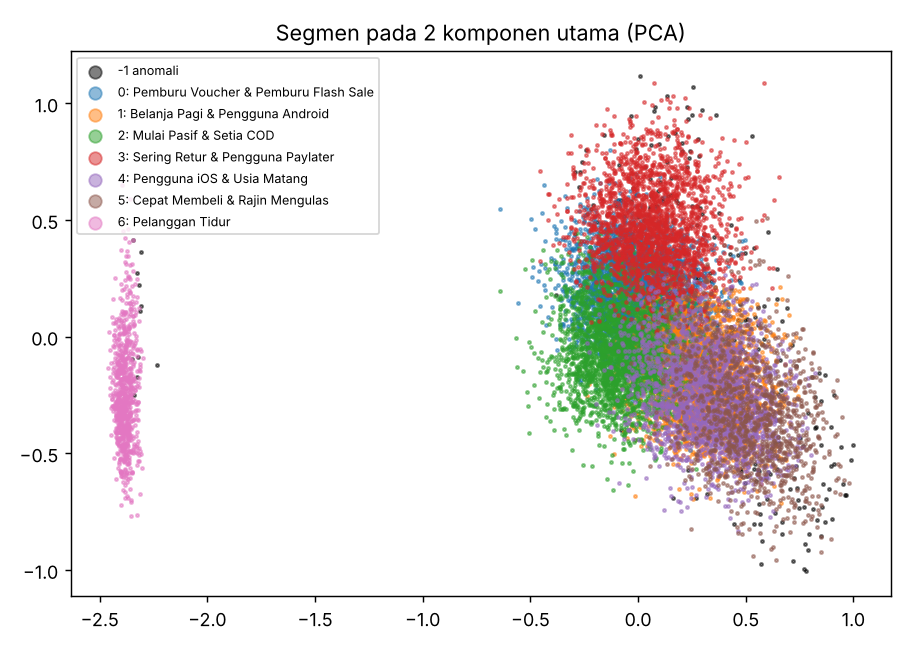
\includegraphics[width=.6\linewidth]{t3_pca.png}
\caption{Tugas 3: segmen pada dua komponen utama.}\label{fig:t3pca}
\end{figure}


\end{document}
